% Chapter Template

\chapter{Evaluation} % Main chapter title

\label{Chapter6} % Change X to a consecutive number; for referencing this chapter elsewhere, use \ref{ChapterX}

\lhead{Chapter 6. \emph{Evaluation}} % Change X to a consecutive
% number; this is for the header on each page - perhaps a shortened title

%----------------------------------------------------------------------------------------
%	SECTION 1
%----------------------------------------------------------------------------------------

\section{Evaluation of Solution}
\label{evaluate_solution}
We have successfully managed to integrate Henshin with the Diagram Predicate
Framework to support exogenous model transformations. We have extended the
Transformation Editor to communicate with the Henshin model transformation
environment. For the solution we have utilized the strengths of the environment
that it implicitly does not support. If we refer back to
figure~\ref{fig:core_metamodel} in section~\ref{integrate_henshin} we saw that
a specification is an instance of a linguistic meta-model that Henshin has no
problem interpreting. The problem arises for the ontological meta-model that
describes the source model. Section ~\ref{Chapter5} describes how we can
explicitly solve this by extending the transformation rules with application
conditions. Henshin utilizes EMF's Ecore modeling system when structuring both
the left hand side and right hand side of a transformation rule. This means
that Henshin supports the 2-layered modeling hierarchy that EMF provides. If we
did not extend the transformation rules with application conditions accordingly
to the DSLs abstraction layer hierarchy, then Henshin would basically interpret
that every DPF model is created accordingly to EMF's 2-layered approach to
meta-modeling. Because Henshin would ignore the different modeling formalisms
provided by several layers of abstraction and threat all modeling elements in a
specification as a node and an arrow. This would lead to a set of transformation
rules that refers to the abstract syntax of the highest abstraction layer that
DPF provides. This is essentially what we want as the target model, but we want
to define the nodes and arrows according to the modeling formalism that is one
abstraction layer higher than the source model and not the highest possible
abstraction layers that is a node with an arrow connected to itself. We
described in the previous section that we can introduce each node and arrow
with its concurrent type from one abstraction layer higher as an application
condition in Henshin. This way Henshin will only locate matches for nodes and
arrows that gives a valid application condition. 


\begin{figure}[H]
	\centering
	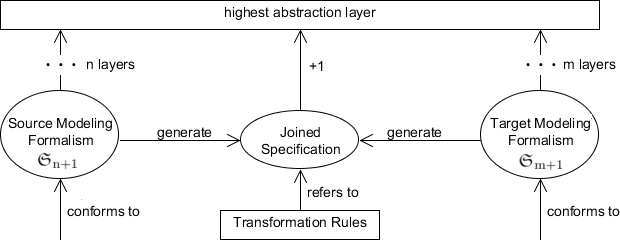
\includegraphics[scale=0.7]{./Figures/simple_modeling_formalism.png}
	\caption[Simplified joined specification]
	{A simplified joined specification that transformation rules refers to.}
	\label{fig:simple_modeling_formalism}
\end{figure}



\section{Future Work}

\subsection{Endogenous Model Transformations}

\subsection{Graphical syntax representation of Transformed models}

\subsection{Making the Model Transformation constraint aware}

%----------------------------------------------------------------------------------------
% SECTION 2
%----------------------------------------------------------------------------------------

\section{Comparison with other editor tools}

In this section we provide a comparison between some model transformation
environments and the Transformation Editor. In our solution we
expanded the Henshin model transformation environment to be able to apply model
transformations to a multi-layered meta-modeling environment like we discussed
in section~\ref{evaluate_solution}. It is natural that the Transformation
Editor will have some similarities to the Henshin environment since our
solutions builds heavily on this environment. But we can still compare our
solution with both Henshin and other transformation tools.

\subsection{Editing Transformation Rules}

In the Transformation Editor we present the transformation rules in a list of
transformation rules. Each transformation rule is extended with a simplified
version of the DPF Editor and a toolbar that contains modeling elements from a
source and a target meta-model. With these modeling elements we can create and
structure a searching pattern and a replacement pattern for each transformation
rules. It is logical that the searching pattern and replacement pattern create
modeling elements that corresponds to the source and target meta-model, since
this is an exogenous model transformation between two different modeling
languages. In Henshin we can choose to create transformation rules in either the
tree based Henshin Model Editor or in a graph based editor. The Transformation
Editor that we created provides an integrated view on transformation rules,
similar to Henshin and GReAT\cite{GReAT}. This means that we do not provide
separate editors to implicitly edit the LHS and the RHS graphs like for
example AGG does. At first glance AGG will most likely provide a more intuitive
approach to editing transformation rules compared to the integrated view that
Henshin and our solution provides. The users needs to understand the principles
behind graph transformations when working with either tools, but AGG might 


AGG was the first tool i encountered, my learning curve became steep after i
learned how graph transformations works. AGG has a clear procedure on how to create and
manage new application rules. AGG is also very intuitive to work with, as long
as the users understands the principles behind graph transformation.
After spending time on AGG and its graphical editor to create transformation rules, the next
stop was Henshin. It was difficult to understand how the principles in graph
transformation works in Henshin. The experience with graph transformation from
AGG was not helpful in the initial hours spent on Henshin. The graphical editor
that AGG and Henshin provides are different in such a way that the creation of
rules are different. Both Henshin and AGG has a tree based editor, but the
editor works differently amongst the two tools, see
figure~\ref{fig:AGGTreeBasedEditor} and~\ref{fig:Henshin_TreeEditor} for the
two editors. The tree based editor for AGG is meant to work as a tool for
browsing through the user created rules, application conditions and graphs. And
for each rule in AGG, the graphical editor opens a left hand side and a right
hand side editing part. This is convenient since editing is now separated in a
left hand and a right hand side window in the graphical editor. The graphical editor can also
add a third editing window, if the user has application conditions attached to a
rule. 

For Henshin this is different, because for this tool the graphical editor
is only an extension to make rule management more intuitive for the users. This
graphical editor is stored in a separate file and is synchronized with the main
henshin file. Changes made to one of these two files is synchronized
accordingly to the other file. The main henshin file contains a tree based
editor that is called Henshin Model Editor. And the Henshin users can create and
apply textual transformation rules in this editor without even initialising the
graphical editor. The graphical editor for Henshin does not implicitly provide
any LHS or RHS for the user to edit their rules in. The users have to know how the tool
performs when using the different action types that Henshin provides. This is
different from AGG, where each rule is provided with an own part for editing
both the LHS and the RHS. The Henshin Model Editor updates the RHS and the LHS
explicitly depending of which action type is provided from the graphical
editor when creating nodes and edges. But other than creating and managing
rules both AGG and Henshin are very similar. They both provide a graphical editor where
the users can insert elements that conform to a meta-model. For AGG these
meta-models are represented as a type graph in the tree based editor. While in
Henshin these meta-models are imported to the Module element in the Henshin Model
Editor and synchronized with the graphical editor file.

The third transformation tool we encountered is ATLAS Transformation Language.
And while this tool is definitely not as intuitive as the two graph
transformation tools, once you understand how to create transformation rules
and how to work with the included meta-models, it is a good framework for
working with model transformations. However, if a user do not fully understand
the Object Constraint Language (OCL), ATL is rather a hard tool to work with.
Because OCL has a very leveled learning curve, since it is a declarative
programming language. Where we are more or less used to work with imperative
programming languages during our studies here in Bergen. ATL provides an editor
where the users can use OCL to create and modify transformation rules. ATL has
a very strict way of writing transformation rules, since the tool uses a
textual based approach to create transformation rules. The user has to use the
predefined stereotypes defined by ATL.



\begin{table}[ht]
\renewcommand*\arraystretch{1.2}
\centering
\begin{tabular}{| c | c | c | c | c |}
\hline
& AGG & Henshin & ATL & DPF Transform \\
\hline
Endogenous transformation & $\surd$ & $\surd$ & $\surd$ & \textcolor{red}{\textbf{---}}\\

Exogenous transformation & $\surd$ & $\surd$ & $\surd$ & $\surd$\\

Input Elements & 1\ldots n & 1\ldots n & 1\ldots n & 1\ldots n\\

Output Elements & 1\ldots n & 1\ldots n & 1\ldots n & 1\ldots n\\

Graphical editor & $\surd$ & $\surd$ & \textcolor{red}{\textbf{---}} & $\surd$
\\

Meta-modeling layers & 2 & 2 & 2 & $\infty$ \\

Separate meta-models & \textcolor{red}{\textbf{---}} &  $\surd$ &  $\surd$ &  $\surd$ \\

Integrated with EMF & \textcolor{red}{\textbf{---}} & $\surd$ & $\surd$ & $\surd$ \\ 

Model transformation file size & 200 kb & 80 kb & 4 kb & 265 kb\\

In-place/out-place transformations & in-place &
in-place & out-place  & out-place \\

\hline
\end{tabular}
\caption{Comparing model transformation tools.}
\label{tab:comparing}
\end{table} 

\subsection{Meta-modeling}

Through defining the abstract syntax is where our editor has its biggest
advantage. The transformation tools that we worked with has a two layered
approach to modeling. First we create the abstract syntax through a meta-model
and second we specify the concrete syntax through a instance model of this
abstract syntax. This is also implicitly true for the Transform Editor, since
every DPF model, regardless of abstraction layer is represented as an instance
model of some abstract syntax model. But this abstract syntax model also
specifies that every DPF model also is an instance of DPF model that are one
abstraction layer higher. So one could say that every DPF model is an instance
of a common modeling language while the abstract syntax for the modeling
elements for this DPF model are typed by another DPF model. With the help of
application conditions we can adapt the Henshin transformation language to make
it possible to apply model transformations to a modeling language that is
specified through an unlimited hierarchy layer of meta-modeling. AGG on the
other hand specifies the abstract syntax in a type graph, that contains both the
source and target meta-model. In AGG we can then create a instance graph that
where modeling elements correspond to modeling elements of the type graph.  

\subsection{Rule Application Control}

The Transformation Editor does not provide the user with any control regarding
how to locate matches and how transformation rules are applied. We generate a
Henshin module that contains a set of transformation rules. We can manipulate
the execution order of these transformation rules, but the algorithm that
Henshin uses to locate matching patterns in a source model is part of the
internal infrastructure of Henshin and cannot be manipulated. We can however
force the transformation rules to be executed in a given order. This version of
the Editor has no support defining a schedule mechanism that specifies how the
rules are applied and will for now only run the transformation rules
sequentially. We can decide the priority of the rules by changing the order
that they appear in the Transformation Editor, but this list will apply rules in
sequential order. Most of the transformation tools open to the public provides
solutions to manipulate the scheduling mechanism, for example ATL provides the
users the possibility to define rules as lazy rules and control how they are
applied. While AGG and the Henshin environment lets the users specify the
scheduling mechanism over a few predefined choices. 

Another thing that is special about our integration of Henshin is that locating
matches are handled differently. An application condition is initially meant to
restrict a transformation rule when locating matches. If application conditions
are not specified for a transformation rule in some 2 layered meta-modeling
transformation tool we will still locate a matching pattern that correspond to
modeling elements that are described in the abstract syntax. The application
condition has a vital role in our integration of Henshin, because the
application conditions are checked against the DPF model that are one
abstraction level higher. Without this application condition we would simply get
a target DPF model that has a list of nodes and arrows that conform to the
highest level of abstraction in DPF. The highest level of abstraction in DPF
is always a node and an arrow, that conforms to itself. So while a 2 layered
meta-modeling transformation tool would find matches in a source model that
correspond to the meta-model, the Transformation Editor would find matches to
the linguistic meta-model and not the ontological meta-model at some level of
abstraction. One could state that an application condition for a 2 layered
meta-modeling transformation tool is independent of the transformation rules
while our version the transformation rules are dependent on the application
conditions to be able to produce a correct target model. 

\subsection{Source - Target Relationship}

The Transformation Editor explicitly performs an out-place model
transformation. This means that we create a target model that is independent of
the source model. For all matching modeling elements we locate in the source
model we create in a target model. We then make sure to specify all the nodes
and arrows with its corresponding type from a specification that is located one
abstraction layer higher. AGG does this differently, since the source and target
model are the same model. Matches are located in the source model, while the
target model is updated in the same model. For an exogenous model transformation
it is required that ATL produce the target model in a separate file. Henshin on
the other hand provides in-place model transformations on the source model. But
when we invoke the Henshin interpreter engine programmatically we can check for
changes before and after exeuting a set of transformation rules. Henshin
transformation engine requires a set of transformation rules, and a graph that
contains the source model. This graph contains a list of all the modeling
elements that are part of the source model. This is why we can explicitly make a
model transformation out-place, by checking this list before and after the
transformation and adding translated elements to a target model. The interpreter
will locate matches in the source model through this graph and produce target
elements to this graph. 

\subsection{Directionality}

To provide a graph based model transformation with the possibility to translate
in both directions is not a simple task. Because then the tool will have to
provide arbitrary switching between source and target models, and therefore the
pattern and replacement graphs will have to be changed when they are switched.
This means that the LHS and the RHS part of a transformation rules have to be
switched out. This is not provided in the Transformation Editor. One could do
this in two steps, to first locate matches in a source model and produce a
target model and then do another model transformation where the source and
target part is switched. Both Henshin and AGG does not provide this since the
corresponding RHS and LHS graphs are created according to the abstract syntax of
the source and target model. 

\subsection{Tracing}

Henshin utilize the generic Trace model to execute an exogenous model
transformation. 

\section{Comparison of the Model Transformation Tools}
\label{comparison}

\subsection{The Editors}
AGG was the first tool i encountered, my learning curve became steep after i
learned how graph transformations works. AGG has a clear procedure on how to create and
manage new application rules. AGG is also very intuitive to work with, as long
as the users understands the principles behind graph transformation.
After spending time on AGG and its graphical editor to create transformation rules, the next
stop was Henshin. It was difficult to understand how the principles in graph
transformation works in Henshin. The experience with graph transformation from
AGG was not helpful in the initial hours spent on Henshin. The graphical editor
that AGG and Henshin provides are different in such a way that the creation of
rules are different. Both Henshin and AGG has a tree based editor, but the
editor works differently amongst the two tools, see
figure~\ref{fig:AGGTreeBasedEditor} and~\ref{fig:Henshin_TreeEditor} for the
two editors. The tree based editor for AGG is meant to work as a tool for
browsing through the user created rules, application conditions and graphs. And
for each rule in AGG, the graphical editor opens a left hand side and a right
hand side editing part. This is convenient since editing is now separated in a
left hand and a right hand side window in the graphical editor. The graphical editor can also
add a third editing window, if the user has application conditions attached to a
rule. 

For Henshin this is different, because for this tool the graphical editor
is only an extension to make rule management more intuitive for the users. This
graphical editor is stored in a separate file and is synchronized with the main
henshin file. Changes made to one of these two files is synchronized
accordingly to the other file. The main henshin file contains a tree based
editor that is called Henshin Model Editor. And the Henshin users can create and
apply textual transformation rules in this editor without even initialising the
graphical editor. The graphical editor for Henshin does not implicitly provide
any LHS or RHS for the user to edit their rules in. The users have to know how the tool
performs when using the different action types that Henshin provides. This is
different from AGG, where each rule is provided with an own part for editing
both the LHS and the RHS. The Henshin Model Editor updates the RHS and the LHS
explicitly depending of which action type is provided from the graphical
editor when creating nodes and edges. But other than creating and managing
rules both AGG and Henshin are very similar. They both provide a graphical editor where
the users can insert elements that conform to a meta-model. For AGG these
meta-models are represented as a type graph in the tree based editor. While in
Henshin these meta-models are imported to the Module element in the Henshin Model
Editor and synchronized with the graphical editor file.

The third transformation tool we encountered is ATLAS Transformation Language.
And while this tool is definitely not as intuitive as the two graph
transformation tools, once you understand how to create transformation rules
and how to work with the included meta-models, it is a good framework for
working with model transformations. However, if a user do not fully understand
the Object Constraint Language (OCL), ATL is rather a hard tool to work with.
Because OCL has a very leveled learning curve, since it is a declarative
programming language. Where we are more or less used to work with imperative
programming languages during our studies here in Bergen. ATL provides an editor
where the users can use OCL to create and modify transformation rules. ATL has
a very strict way of writing transformation rules, since the tool uses a
textual based approach to create transformation rules. The user has to use the
predefined stereotypes defined by ATL.

\subsection{The Meta-models}
Meta-models are initialised and handled differently amongst some of the tools.
The initialisation of the meta-models for Henshin and ATL is similar. Both of
these tools use Ecore to create meta-models, since they are both integrated with
EMF. For Henshin and ATL the user has to create one Ecore model for both the
source and the target meta-model. Both of these meta-models can be imported both
into Henshin and ATL. One thing that is convenient with Henshin that ATL does
not provide, is that Henshin provides a list of meta-models that is available
for the user. These are meta-models that can be used either as source or target
meta-model. If we want to translate a instance model to an Ecore model, we can
in Henshin import this ecore meta-model from a list and use it as the target meta-model.

Unlike Henshin and ATL, AGG does not allow for separately initialisation of
meta-models. For AGG we have to create both the target and source meta-model in a
disjoint meta-model, or one common type graph in AGG.

The user has to fill out a configuration form for an ATL model transformation.
This form the user has to explicitly assign the meta-models to source model and
target models. The run configuration is done prior to the execution of the model
to model transformation. In Henshin the user has to implicit include the
meta-models in the Henshin module element. Henshin will not allow the user to
create nodes or create edges between nodes that are not defined in the
meta-models. 

AGG on the other hand uses a disjoint meta-model. This means that in AGG there
is something called a type graph, and in this type graph both the target and
the source meta-model are defined. AGG handles consistency similar to
Henshin. AGG will restrict the user to only create nodes or arrows between
nodes that are specified in the type graph. Figure \ref{fig:AggTypeGraph}
in chapter 3 shows that there are created references between two meta-models. And
through the use of these references, AGG can create and modify application
rules to translate these two models represented in the type graph. 
 
\subsection{Transformation Rules}
We have seen that the creation of transformation rules varies over the three
different tools. ATL provides a textual based approach and therefore requires
multiple lines of code. The abstract syntax for the three different tools are
not that different, since both Henshin and ATL utilizes the Ecore model to
create meta-models and AGG creates one type graph that contains the abstract
syntax for both the source and target model. The abstract syntax can be
visualized either by using the tree based model editor that EMF provides or by
using a tird party tool for a graphical representation of the models. The
concrete syntax are obviously different between the three tools. AGG and Henshin
provides a concrete graphical syntax, while ATL on the other side provides a
concrete textual syntax for creating and modifying transformation rules. For
both AGG and Henshin the rules can be created and modified by using a graphical
editor. AGG separates the RHS and the LHS in two separate editing parts while
Henshin use predefined word sequences to distinguish the two different sides.
If the rules are quite large, with multiple nodes and arrows the rules
presented in Henshin becomes easier to read and maintain. But both AGG and
Henshin has a clear way of representing the rules and possible attached
application conditions. All three tools have a left hand side
and a right hand side, but are represented differently amongst the rules.
Henshin and AGG use graph patterns to represent the LHS and the RHS while ATL
utilizes logical expressions. In section 3 we discussed that ATL can have both
declarative and imperative transformation rules. In Henshin and AGG the LHS and
the RHS are represented as graphs. Where the LHS represents the pattern graph
that is matched for an instance model and the RHS represents the part that should be
replaced for the instance model. For ATL the LHS represents the source model
while the RHS represents the target model. 

Both AGG and Henshin can specify both negative and positive application
conditions. These are attached to pattern graph or the LHS of a rule. These
application conditions provides a true or false clause that can be used to
restrict the pattern graph. For ATL these conditions are handled by OCL
expressions, where one example is the if-then clause.

\subsection{Relationship between Source and Target}
For an exogenous transformation in ATL it is mandatory to create a new target
that holds all the target model elements. Exogenous model transformation in ATL
is therefore called an out-place transformations. In AGG on the other hand both
source and target model is always the same model. This means that AGG performs an
in-place update on its original source model. Henshin is a bit more special,
because implicitly it performs in-place update on the source model. But in
Henshin you can initialize variables that explicitly captures the transformed
target elements and save these to a separate file in your storage unit. Note
however, that this can only be done when utilizing the Henshin interpreter
programmatically. 

\subsection{Rule Scheduling}

ATL does the scheduling implicit, where the user has no control over the
scheduling algorithm defined by the tool. The user can however influence the scheduling
algorithm defined by the ATL transformation engine by designing the logic in the
transformation rules to apply in a certain order. The transformation
engine will first execute the declarative rules before applying the imperative
section of a transformation rule. AGG and Henshin does however, give the
users the possibility to influence how the transformation rules are applied. 
In Henshin and AGG this is handled explicitly before applying the transformation
rules, where the user can change the execution order of the rule.
For example the rules can be applied non-deterministically or by forcing the
transformation rules to be applied in a sequential order. To force the
transformation in a sequential order could result in performance issues compared
to applying the rules non-deterministically. AGG provides the users with the
possibility to organize the transformation process into several phases or
layers. These layers are numbered from 0 \ldots n, and the lower the number the
higher the priority for the rule, when it is translated. This gives the users
the possibility to execute rules layer by layer. In Henshin these rule scheduling
mechanisms are referred to as transformation units. For this tool it is possible
to specify units that supports rule iteration, both by looping through rules
until there are no more changes detected or by iterating through rules for a
fixed number of iterations. In Henshin it is also possible to specify an
amalgamation unit, that is an unit that provides a forall-operation for the
matching pattern graph. This unit has a kernel rule and multiple underlying
rules that are matched as often as possible. This amalgamation unit can be
compared to a for loop in Java. It is clear that Henshin provides the users with
quite an variety of controlling the execution of rules.

\subsection{Rule Organization}

ATL organizes the transformation rules inside modules, and its therefore easy to
reuse these modules if applicable. This is convenient for
users of ATL since this means that all created rules can be used to form new
transformation rules. Henshin provides the user with the possibility to nest or 
reuse rules in different scheduling mechanism or transformation units
as we discussed in the last paragraph. But Henshin and AGG does however not
provide the user with the possibility to reuse rules in the creation of new
rules as ATL does. 

\subsection{Tracing}

Tracing in the three tools provides a unique link
between a source and a target. The source represents the matched part while the
target represents the generated or replacement part. All three tools provides
dedicated support for traceability. But these traceable links are handled
differently amongst the tools. For ATL the trace model works as a storage
location and automatically creates trace links between source and target
elements. These traceable links are internally used by the ATL
transformation engine when executing a model transformation. But we explained in
section 3 that these trace links can be explicitly captured by creating
transformation rules that generates a collection of trace links in a
separate trace file. Henshin does this differently, because tracing is
controlled by the users. Henshin has a dedicated Trace Model that can be
imported to the Henshin module as an Ecore model. The trace model in Henshin
are automatically created when executing rules, but the user have to manually
assign the traceable links inside the transformation rules. The traces in
Henshin are translated when a rule is executed, and therefore the user has to
be aware of this when using these traces in other rules, since this
could lead to the creation of multiple traceable links between the same
elements. Tracing in AGG plays a vital role to executing model transformations.
Traceable elements are created similar to any other elements when initializing
the type graph. With traceable links between the source and the
target elements, AGG can be certain that elements are transformed. The traceable
link in AGG ensures that a match in the pattern graph is only matched once. If we do
not create a traceable link between source and target elements in AGG, the
rules will be applied an endless amount of times. Tracing amongst the three
different tools are different in such a way that it is required for exogenous
model transformations for AGG and ATL. In ATL the traceable links are created
automatically and cannot be controlled by the users, while in AGG the traceable
links are created as bridges between source and target elements. For Henshin
the Trace model is optional. 

\subsection{Directionality}

Its clear to see that all three tools are unidirectional, since they can be
executed in one direction only. And that is to compute a target model from a
source model. The three tools requires two model transformations to be able to
transform in multiple directions. Where the source and target model and
meta-models switch places. But this is not how multidirectional transformations
work. A multidirectional transformation can execute in both direction when
performing a model transformation.

\begin{table}[ht]
\centering
\begin{tabular}{| c | c | c | c |}
\hline
 & AGG & Henshin & ATL \\
\hline
Endogenous transformation & \cellcolor{green!25}Yes &
\cellcolor{green!25}Yes & \cellcolor{green!25}Yes \\

Exogenous transformation & \cellcolor{green!25}Yes &
\cellcolor{green!25}Yes & \cellcolor{green!25}Yes \\

Input Elements & 1\ldots n & 1\ldots n & 1\ldots n\\
Output Elements & 1\ldots n & 1\ldots n & 1\ldots n\\
Graphical editor &\cellcolor{green!25}Yes &
\cellcolor{green!25}Yes &\cellcolor{red!25}No  \\
Integrated with Java & \cellcolor{green!25}Yes &
\cellcolor{green!25}Yes & \cellcolor{green!25}Yes \\
Separate meta-models & \cellcolor{red!25}No &
\cellcolor{green!25}Yes & \cellcolor{green!25}Yes \\
Integrated with EMF & \cellcolor{red!25}No &
\cellcolor{green!25}Yes & \cellcolor{green!25}Yes \\
Model transformation file size &200 kb &80 kb &4 kb \\
In-place/out-place model transformation &in-place &
in-place &out-place \\
\hline

\end{tabular}
\caption [Comparing model transformation tools]
{Comparing model transformation tools.}
\end{table}

\newpage




From the table above, we can see that all the three tools have support
for both endogenous and exogenous model transformations. 

All the three tools has support for an arbitrary number of both input and
output elements. This means that if the tool takes a number of input models, then it
produces the same number of target models. Take an ATL module as an example. It
accepts a fixed number of models as input, and returns a fixed number of target
models. This means that an ATL module can not generate an unknown number of
target models. If there is one input model, then there will be one output model
that conforms to a target meta-model.

Both AGG and Henshin provides a graphical editor, where the users can create and
modify transformation rules. This makes them both very intuitive for the users.
This is not the case for ATL, which uses a textual based approach. For ATL the
users have to implement transformation rules in programming code.

All three tools can be integrated with Java. For Henshin and ATL the files
containing the transformation rules have to be created before they can be used
in a java application. In ATL this has to be a ``atl'' file containing a ATL
module that has a list of rules. This is because the ATL transformation engine
relies on a file extension with the name ``atl''.

One thing that is worth mentioning is that AGG does not support the Eclipse
Modeling Framework. In EMF the root of all modeling objects is called
EObject. And this EObject has no references to the Java Object. Therefore AGG
can not be integrated with EMF, since AGG can take Java Objects as input,
but not EObjects. Both Henshin and ATL supports EMF. This means that the user
can use the EMF API together with Henshin and ATL in a Java Application.

We can also se that the size of the transformation rules is different
between the three tools. A classic example of an exogenous transformation is
translating from a class diagram to a relational database, that has more or less become a
benchmark for model to model transformations. For this example we can see that
AGG uses 200 kb of the storage space. This number is so unbelievable small
that it will never be noticed in any modern computers. But there is one
interesting thing however, and that is that the transformation rules defined in
ATL is 50 times smaller than AGG. What this basically means is that creating model
transformations through the use of textual concrete syntax is less space
consuming than through the use of graphical syntax. This is only logical since
the graphical syntax based transformation languages requires more storage
space simply because they use graphical elements to represent the transformation
rules.

\subsection{Translating the instance model}

When ATL transformation language executes the application rules for the model to
model transformation, a new model instance is created for the target model. This
means that the source model is independent of the target model. Where Henshin
and AGG performs in-place model to model transformations. This means that they
both operate on an instance model of the source meta-model, and translates
inside this instance model. All three approaches can however give the same
result. Inn AGG and Henshin the users just need to make sure to delete unwanted
elements from the translated host graph. On the other side, for ATL this is not
needed, since both the source and target model are kept as separated files. This
is also possible to achieve with Henshin. If the user programmatically invoke
the Henshin Interpreter the target model can be forced to be saved in a newly
created file. Henshin will still do an in-place model transformation, but it is
possible to save the translated object in a separate file. It is then possible
to perform an in-place transformation in Henshin while saving the target
instance model in a separate file. 

\section{Conclusion}

Now that we have extended the DPF workbench environment with an early version
that supports model to model transformations.

We have experienced that after working with the three tools that in the initial
learning phase both AGG and Henshin seems to be more intuitive to use because of the
graphical editor they provide. Because of the extensive language OCL, ATL
requires more hours to understand compared to AGG and Henshin. Its important to
take into consideration that I have read through papers that explain the
principles behind graph transformations. This makes it easier to understand how
AGG and Henshin introduces the users to model transformation, even though both
tools have different solutions to how graph transformation is implemented. But
learning a new programming language requires time. And therefore a graphical
solution might feel more intuitive then a textual solution. However I also know
that if you master a programming language, then writing code is more productive
compared to using a graphical editor. Therefore if the user master both the ATL
transformation language and the OCL programming language then it might be a
productive way of creating transformation rules. All these three tools have gone
through several iterations and releases and also have received feedback from the
user community. This only reassure me that all these three tools are viable
choices for model transformations. Most of the hours have been spent on
Henshin's working with the graphical editor and programmatically
invoking the Henshin interpreter. The graphical editor provides a clear
process of defining new transformation rules once I understood how the graph
transformation principles worked for Henshin. The Henshin Interpreter has
an extensive API that can be used to programmatically translate the
models. The interpreter still requires a set of Henshin rules to be able to
initiate a model transformation, but this means that the user can create its own
graphical editor and integrate this editor with Henshin to manipulate models.
Together with the Henshin Model Editor, the graphical editor and the Henshin
Interpreter Henshin provides a very viable transformation language for model
